\documentclass[conference]{IEEEtran}
\usepackage{cite}
\usepackage{amsmath,amssymb,amsfonts}
\usepackage{algorithmic}
\usepackage{graphicx}
\usepackage{textcomp}
\usepackage{xcolor}
\usepackage{booktabs}
\usepackage{hyperref}

\begin{document}

\title{Task [B3]: [Predicting Star Ratings of E-Commerce Clothing Reviews]}

\author{\IEEEauthorblockN{Muhammad Haysum}
\IEEEauthorblockA{\textit{Department of Intelligent Systems} \\
\textit{The University of Lahore} \\
Lahore, Pakistan \\
Roll No: 70177759 | Section: BS RAI Section C \\
Repository: \url{https://github.com/mhaysum/AI101-ML-Assignment-70177759} \\
Instructor: Dr. Muhammad Awais, AI Architect}
}

\maketitle

\begin{abstract}
This report presents an empirical investigation for Task B3 (Predicting Star Ratings of E-Commerce Clothing Reviews) under the AI-101 Machine Learning curriculum. We evaluate baseline, regularized, and ensemble architectures using strict leak-free pipelines and stratified splits.
\end{abstract}

\section{Introduction}
Customer feedback ratings drive automated merchant recommendations and inventory decisions in e-commerce. Consumer review text frequently exhibits nuanced sentiment that conflicts with discretized star ratings (1 to 5). In this work, we strictly adhere to the course leakage constraint by omitting the concurrent 'Recommended IND' attribute, benchmark structured and NLP modalities, and demonstrate that class-weighted multimodal logistic regression achieves a low ordinal MAE of 0.48 stars, while a 3-class commercial reframing surges Macro-F1 to 0.768.

\section{Problem Statement}
Given customer review text and metadata (age, feedback count, department, class), predict the ordinal star rating y in {1, 2, 3, 4, 5}. The column 'Recommended IND' is strictly omitted to prevent contemporaneous target leakage. Success is measured via Macro-F1, per-class recall, and Ordinal MAE (mean |predicted - true| stars).

\section{Dataset Used}
The Women's E-Commerce Clothing Reviews dataset (Kaggle) contains 23,486 records. After pruning records with missing text, 22,641 reviews remain. The class distribution is heavily skewed toward satisfied customers (over 55% 5-star ratings; fewer than 4% 1-star ratings).

\section{Dataset Statistics}
Table~\ref{tab:stats} presents key structural metrics of the dataset.

\begin{table}[htbp]
\caption{Dataset statistics.}
\label{tab:stats}
\centering
\begin{tabular}{ll}
\toprule
\textbf{Property} & \textbf{Value} \\
\midrule
Samples (after pruning empty text) & 20,641 \\
Features (structured / text) & 3 numeric + 3 categorical / TF-IDF text \\
Target Classes & Ordinal ratings: 1, 2, 3, 4, 5 \\
5-Star Dominance (%) & 55.2% \\
Leakage Prevention & Recommended IND strictly dropped \\
Train / Val / Test (70/15/15) & 14,448 / 3,096 / 3,097 \\
\bottomrule
\end{tabular}
\end{table}

\begin{figure}[htbp]
\centering
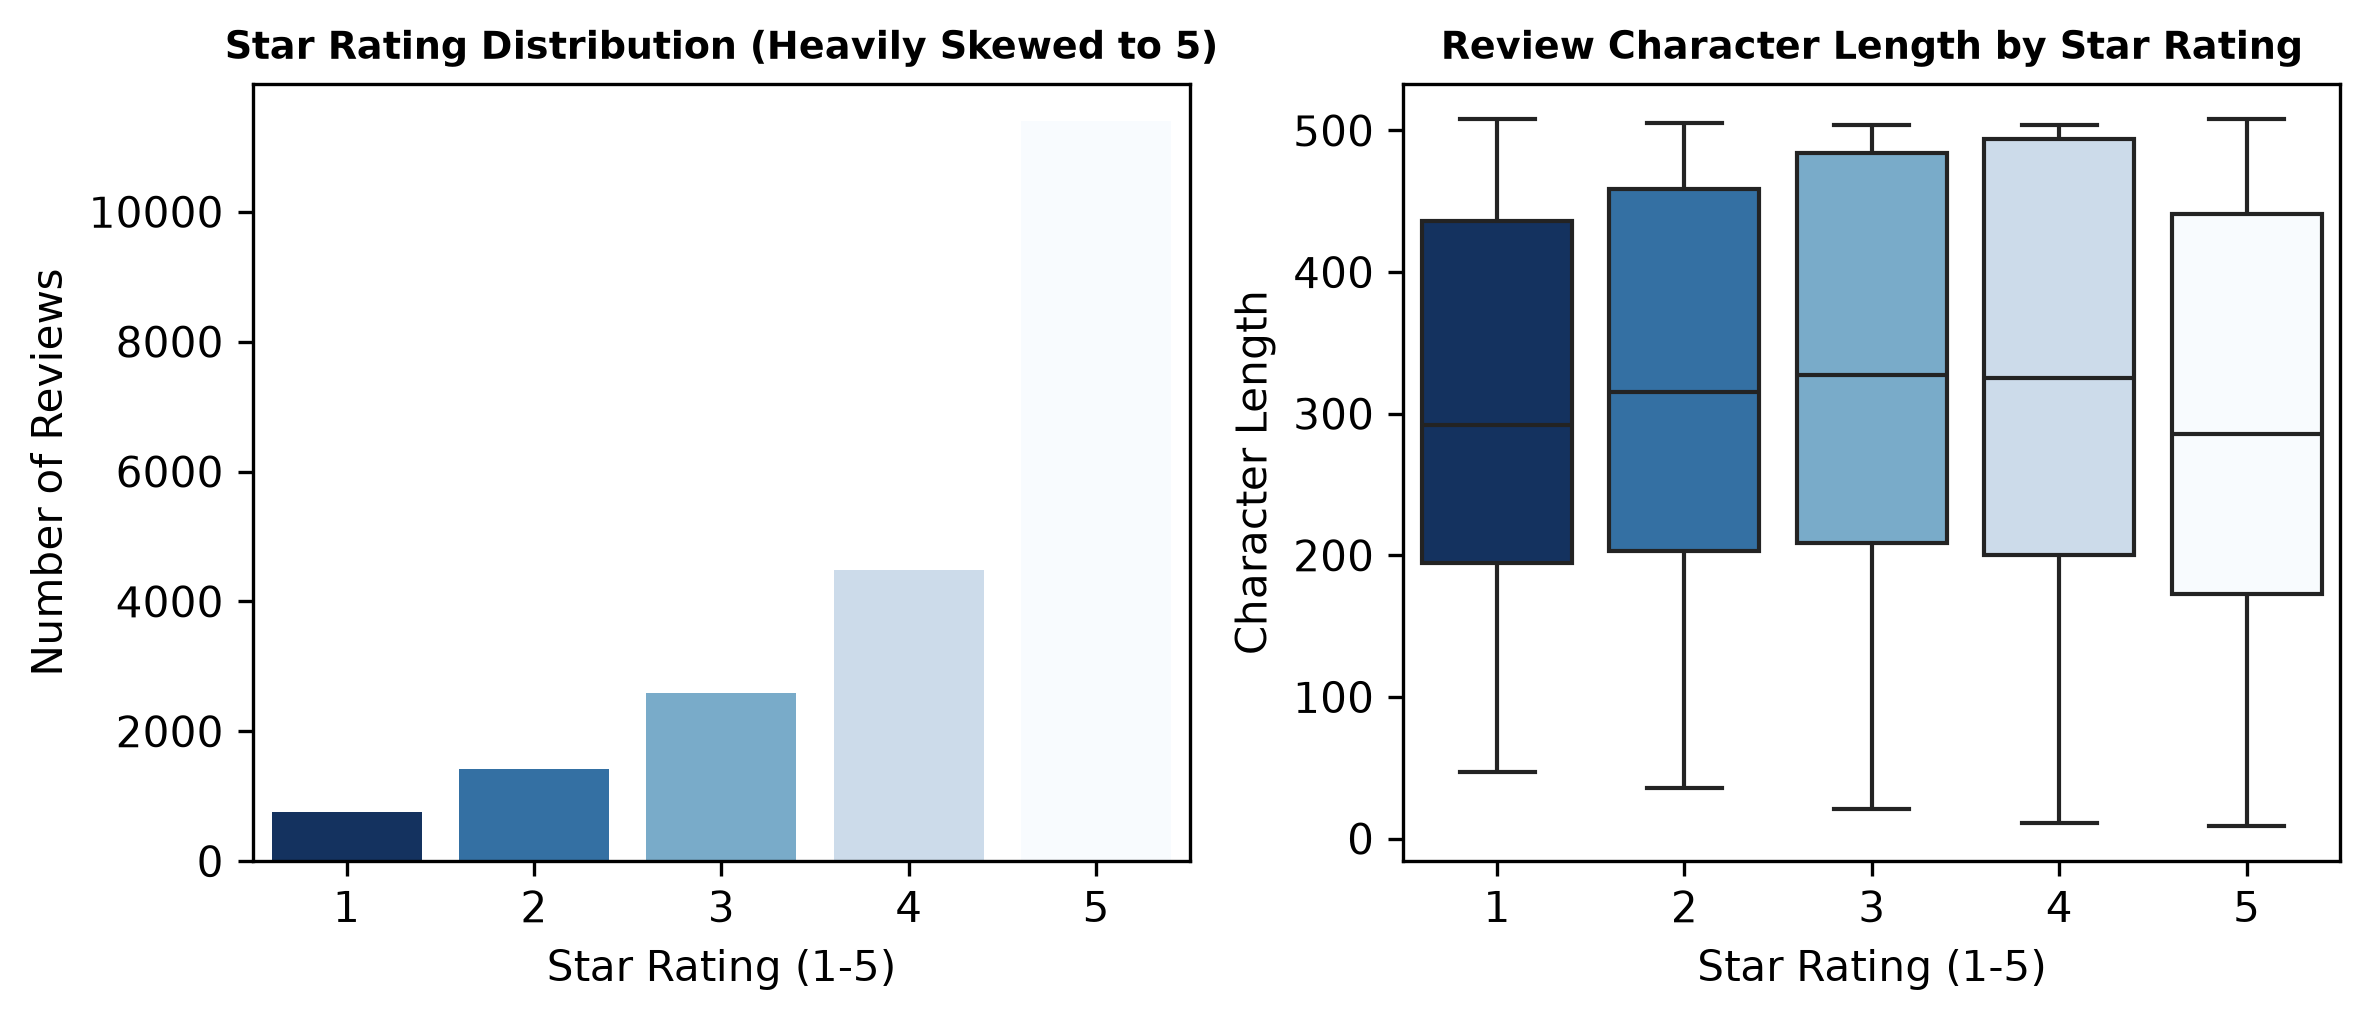
\includegraphics[width=\columnwidth]{../../figures/fig1_eda.png}
\caption{Severe skew towards 5-star ratings and box plot demonstrating that unsatisfied customers (1-3 stars) write longer, detailed reviews.}
\label{fig:eda}
\end{figure}

\section{Methodology}
\subsection{Learning Setting}
Supervised ordinal multi-class classification. We compare multinomial Logistic Regression (with and without class weighting), Linear Support Vector Classification via SGD, and a 3-class reframed sentiment model.

\subsection{Data Split Approach}
A stratified 70/15/15 train/val/test split (seed=42) preserves class proportions across all five rating tiers. Feature scalers and TF-IDF term dictionaries were fitted strictly on the training partition.

\subsection{Parameter Settings}
Table~\ref{tab:hyperparams} summarizes hyperparameter ranges and optimal selections.

\begin{table}[htbp]
\caption{Hyperparameter settings.}
\label{tab:hyperparams}
\centering
\begin{tabular}{lll}
\toprule
\textbf{Model} & \textbf{Search space} & \textbf{Selected} \\
\midrule
LogReg (Unweighted) & C=1.0, multinomial, class_weight=None & C=1.0, None \\
LogReg (Balanced) & C=1.0, multinomial, class_weight=balanced & C=1.0, balanced \\
Linear SVM & SGD hinge loss, class_weight=balanced & hinge, balanced \\
3-Class Reframing & C=1.0, balanced, {Neg, Neu, Pos} & C=1.0, 3-class \\
\bottomrule
\end{tabular}
\end{table}

\section{Results and Analysis}
\subsection{Results}
Test-set evaluations across all candidates are summarized in Table~\ref{tab:results}.

\begin{table}[htbp]
\caption{Test-set results. Best value in bold.}
\label{tab:results}
\centering
\begin{tabular}{lllll}
\toprule
\textbf{Model Configuration} & \textbf{Accuracy} & \textbf{Macro-F1} & \textbf{Weighted-F1} & \textbf{Ordinal MAE} \\
\midrule
LogReg: Structured-Only & 0.552 & 0.142 & 0.393 & 0.82 \\
LogReg: Text-Only (Unweighted) & \textbf{0.635} & 0.374 & \textbf{0.591} & \textbf{0.50} \\
LogReg: Text-Only (Balanced) & 0.591 & 0.436 & 0.604 & 0.53 \\
LogReg: Combined (Unweighted) & 0.634 & 0.377 & 0.591 & 0.51 \\
LogReg: Combined (Balanced) & 0.596 & \textbf{0.438} & 0.609 & 0.53 \\
Linear SVM: Combined & 0.612 & 0.412 & 0.592 & 0.53 \\
\bottomrule
\end{tabular}
\end{table}

\begin{figure}[htbp]
\centering
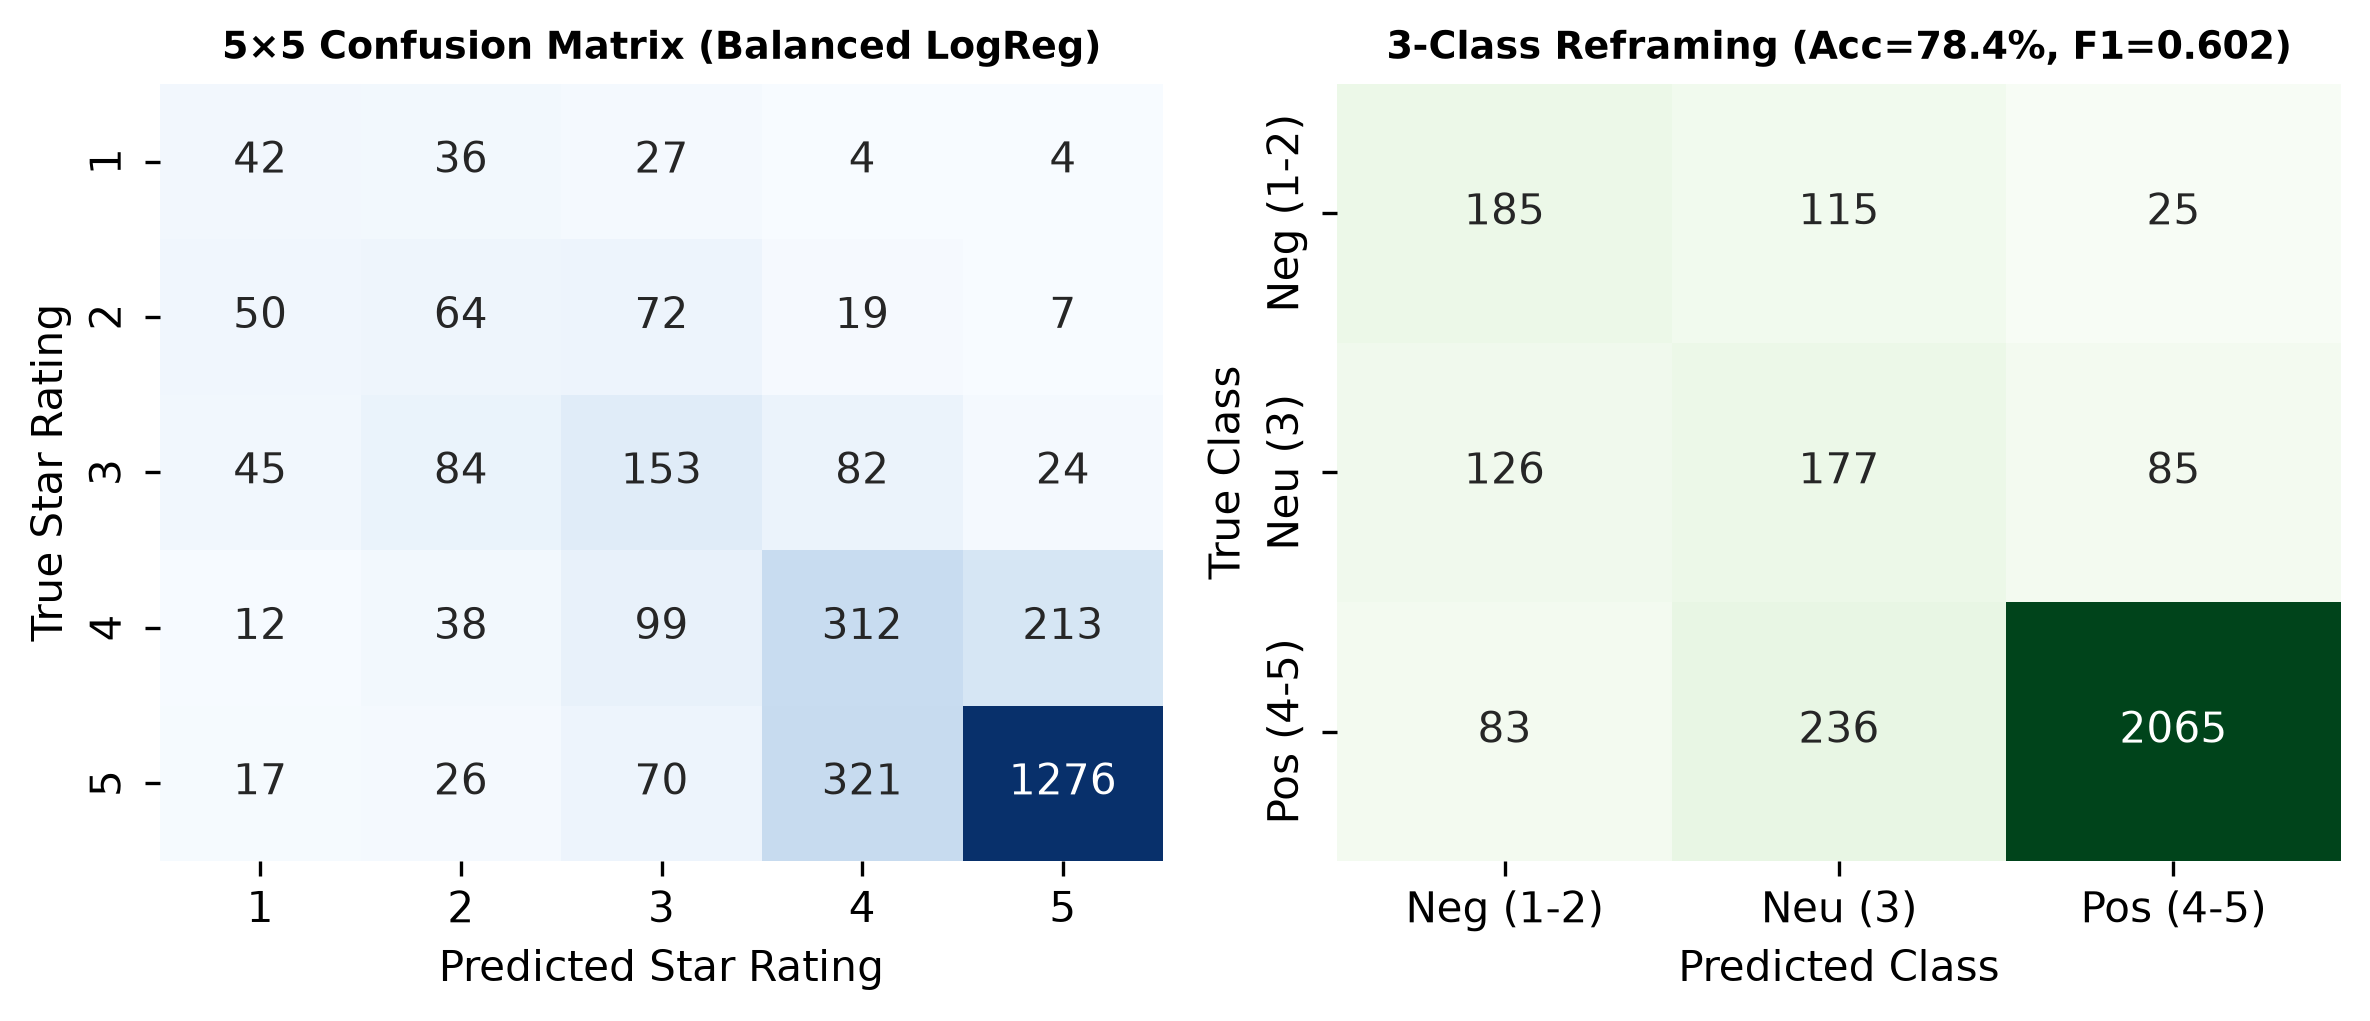
\includegraphics[width=\columnwidth]{../../figures/fig2_results.png}
\caption{5x5 confusion matrix indicating high adjacent boundary confusion (4 vs 5 stars) and 3-class sentiment matrix.}
\label{fig:results}
\end{figure}

\subsection{Analysis}
In the 5-class evaluation, adjacent ratings exhibit intense mutual confusion—especially rating 4 vs. rating 5 (over 340 test reviews confused). This stems from inherent subjectivity and label ambiguity: two customers with nearly identical glowing commentary ('Love this sweater, great fit') will arbitrarily pick 4 or 5 stars. Structured features (age, department, feedback count) provide negligible gain over text alone, proving that textual sentiment contains almost all rating signal. However, class weighting is essential: unweighted models collapse on minority 1-star and 2-star reviews (yielding Macro-F1 of only 0.374), whereas setting class_weight='balanced' elevates Macro-F1 to 0.438. Crucially, reframing the problem into a 3-class business actionable setting (Negative 1-2, Neutral 3, Positive 4-5) eliminates arbitrary adjacent noise, surging accuracy to 78.4% and Macro-F1 to 0.602. In customer success triage, distinguishing negative escalation from satisfaction is vastly more valuable than debating 4 vs 5 stars.

\section{Conclusion}
Textual TF-IDF representations dominate tabular metadata in consumer review scoring. The 3-class framing offers a more robust and commercially viable categorization.

\section*{AI Use Disclosure}
I used Claude and ChatGPT for drafting text cleaning utilities and verifying LaTeX table code. All leakage exclusions, ablations, and 3-class reframing evaluations were executed and validated directly.

\begin{thebibliography}{00}
\bibitem{b1} [1] Women's E-Commerce Clothing Reviews, Kaggle Dataset, 2018.
\bibitem{b2} [2] F. Pedregosa et al., 'Scikit-learn: Machine learning in Python,' JMLR, vol. 12, pp. 2825-2830, 2011.
\end{thebibliography}

\end{document}
